\documentclass[12pt]{article}
\usepackage{tikz}
\pagestyle{empty}
\begin{document}
\begin{tikzpicture}[x=1cm,y=1cm]
\path (0,0) -- (2,0);
\end{tikzpicture}
\newpage
\begin{tikzpicture}[x=1cm,y=1cm]
\path[red] (0,0) -- (2,0);
\end{tikzpicture}
\newpage
\begin{tikzpicture}[x=1cm,y=1cm]
\path[->] (0,0) -- (2,0);
\end{tikzpicture}
\newpage
\begin{tikzpicture}[x=1cm,y=1cm]
\path[red,->] (0,0) -- (2,0);
\end{tikzpicture}
\newpage
\begin{tikzpicture}[x=1cm,y=1cm]
\path[draw] (0,0) -- (2,0);
\end{tikzpicture}
\newpage
\begin{tikzpicture}[x=1cm,y=1cm]
\path[draw=red] (0,0) -- (2,0);
\end{tikzpicture}
\newpage
\begin{tikzpicture}[x=1cm,y=1cm]
\draw (0,0) -- (2,0);
\end{tikzpicture}
\newpage
\begin{tikzpicture}[x=1cm,y=1cm]
\draw[red] (0,0) -- (2,0);
\end{tikzpicture}
\newpage
\begin{tikzpicture}[x=1cm,y=1cm]
\draw[->] (0,0) -- (2,0);
\end{tikzpicture}
\newpage
\begin{tikzpicture}[x=1cm,y=1cm]
\draw[draw=none] (0,0) -- (2,0);
\end{tikzpicture}
\newpage
\begin{tikzpicture}[x=1cm,y=1cm]
\path (0,0) circle (4pt);
\end{tikzpicture}
\newpage

\begin{tikzpicture}[x=1cm,y=1cm]
\path[fill=red] (0,0) circle (4pt);
\end{tikzpicture}
\newpage

\begin{tikzpicture}[x=1cm,y=1cm]
\path[draw,fill=red] (0,0) circle (4pt);
\end{tikzpicture}
\newpage

\begin{tikzpicture}[x=1cm,y=1cm]
\fill[red] (0,0) circle (4pt);
\end{tikzpicture}
\newpage

\begin{tikzpicture}[x=1cm,y=1cm]
\fill (0,0) rectangle (2,1);
\end{tikzpicture}
\newpage
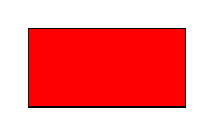
\begin{tikzpicture}[x=1cm,y=1cm]
\draw[fill=red] (0,0) rectangle (2,1);
\end{tikzpicture}
\newpage

\begin{tikzpicture}[x=1cm,y=1cm]
\filldraw[red] (0,0) circle (4pt);
\end{tikzpicture}
\newpage

\begin{tikzpicture}[x=1cm,y=1cm]
\draw[red,line width=2pt] (0,0) -- (2,0);
\end{tikzpicture}
\end{document}
